% 6.344 (Digital Image Processing) Final Project
% Author: Michael Mekonnen

\documentclass[12pt]{amsart}

% Packages
\usepackage[margin=1.5in]{geometry}
\usepackage[pdftex]{graphicx}
\usepackage{hyperref}
\usepackage[usenames,dvipsnames]{xcolor}

% Custom commands
\newcommand{\HRule}{\rule{\linewidth}{0.5mm}}

% Colors
\definecolor{light-gray}{gray}{0.65}

\title{Edge Detection}

\begin{document}

\begin{titlepage}
\begin{center}

\textsc{\LARGE Massachusetts Institute of Technology}\\[1.5cm]

\vspace{4cm}

\textsc{\Large Digital Image Processing (6.344) \\ Final Project}\\[0.5cm]

\HRule \\[0.4cm]
{ \huge \bfseries Edge Detection}\\[0.4cm]
\HRule \\[1.5cm]

\large Michael \textsc{Mekonnen}

\vfill

{\large \today}

\end{center}
\end{titlepage}

\maketitle

\section{Introduction}

For my 6.344 final project, I took up the task of edge detection: given an image, produce a new image that clearly outlines the edges in the original image. This is a well studied idea, and there are various methods available. Here, I will explore two of the most widely used methods: the gradient-based method and the laplacian-based method.

\section{Gradient-based method}

The gradient-based method detects edges in a $2D$ image by finding the analogue of a gradient for the image and then finding the peaks of the magnitude of the gradient. It helps to think about this in $1D$. To find the ``edges" of a $1D$ continuous signal $f(x)$, we would first take the derivative $\frac{df}{dx}$ and look for it's optima since an edge in $1D$ is a fast change in $f(x)$ for a small change in $x$, which is we can very clearly detect by taking the derivative. For a $2D$ continuous signal $f(x,y)$, we can do a very similar thing. Here, we would find the magnitude of the gradient given by $|\nabla f| = \sqrt{(\frac{\partial f}{\partial x})^2 + (\frac{\partial f}{\partial y})^2}$ and search for its optima. When we are working with a digital image, we are not able to take derivatives, so we approximate the derivatives. There are various ways to approximate the derivatives $\frac{\partial f}{\partial x}$ and $\frac{\partial f}{\partial y}$, but one intuitive and standard method is to use filters like the ones shown in Figure \ref{fig:derivativefilters}.

In Figure \ref{fig:gradientmethod}, I present my overall gradient-based edge detection system. Given an image $f(n_1, n_2)$, we first finds its derivatives in the $n_1$ and $n_2$ directions exactly by using the filters shown in Figure \ref{fig:derivativefilters}. Next, we compute an approximation of the magnitude of the gradient by taking the square root of the sum of the squares of the two different derivatives. The standard gradient-based edge detection method then proceeds to finding the pixels whose gradient magnitude exceeds some threshold, and these pixels are classified as edge pixels. This step is usually followed by an edge-thinning step. The choice of this threshold depends on the particular image at hand. In my project, I chose to do something different from using an experimentally found threshold. I first find the $95^{th}$ percentile gradient magnitude, $M$. Then, for a given pixel $(n_1, n_2)$, I set its brightness level in the output image to be:
\begin{equation*}
255 \left(1 - \left(\frac{|\nabla f(n_1, n_2)|}{M}\right)^\alpha\right).
\end{equation*}
What this does is assign pixels whose gradient magnitude is ``high" (i.e. close to $M$) a low brightness (close to $0$ or black) and assign pixels whose gradient magnitude is ``low" (i.e. close to $0$) a high brightness (close to $255$ or white). $\alpha > 0$ is simply a tuning parameter. The resulting edge map traces the edges in the image, and highlights the more drastic edges more strongly. One important benefit of this method is that it avoids having to manually pick a threshold value for each image of interest. There is still the task of choosing the right value of $\alpha$, but I have observed from experimentation that the same value of $\alpha$ has a uniform effect over different images, so one may choose some default value of $\alpha$, for example $2$, and still obtain a reasonable result for various images. Another advantage of using this method of assigning brightness in the edge-map image is that it avoids discontinuities in places where there are edges that are not highly pronounced. Finally, this method avoids the need for edge-thinning.

\begin{figure}
\begin{minipage}[b]{0.45\linewidth}
\centering
\begin{tabular}{c || c | c | c }
 {\color{light-gray}1} & -1 & 0 & 1 \\
\hline
 {\color{light-gray}0} & -1 & 0 & 1 \\
\hline
 {\color{light-gray}-1} & -1 & 0 & 1 \\
\hline\hline
& {\color{light-gray}-1} & {\color{light-gray}0} & {\color{light-gray}1} \\
\end{tabular}
\end{minipage}
\hspace{0.5cm}
\begin{minipage}[b]{0.45\linewidth}
\centering
\begin{tabular}{c || c | c | c }
 {\color{light-gray}1} & 1 & 1 & 1 \\
\hline
 {\color{light-gray}0} & 0 & 0 & 0 \\
\hline
 {\color{light-gray}-1} & -1 & -1 & -1 \\
\hline\hline
& {\color{light-gray}-1} & {\color{light-gray}0} & {\color{light-gray}1} \\
\end{tabular}
\end{minipage}
\caption{LTI filters to approximate derivatives of a $2D$ discrete signal, in the $n_1$ and $n_2$ directions respectively.}
\label{fig:derivativefilters}
\end{figure}

\begin{figure}
\centering
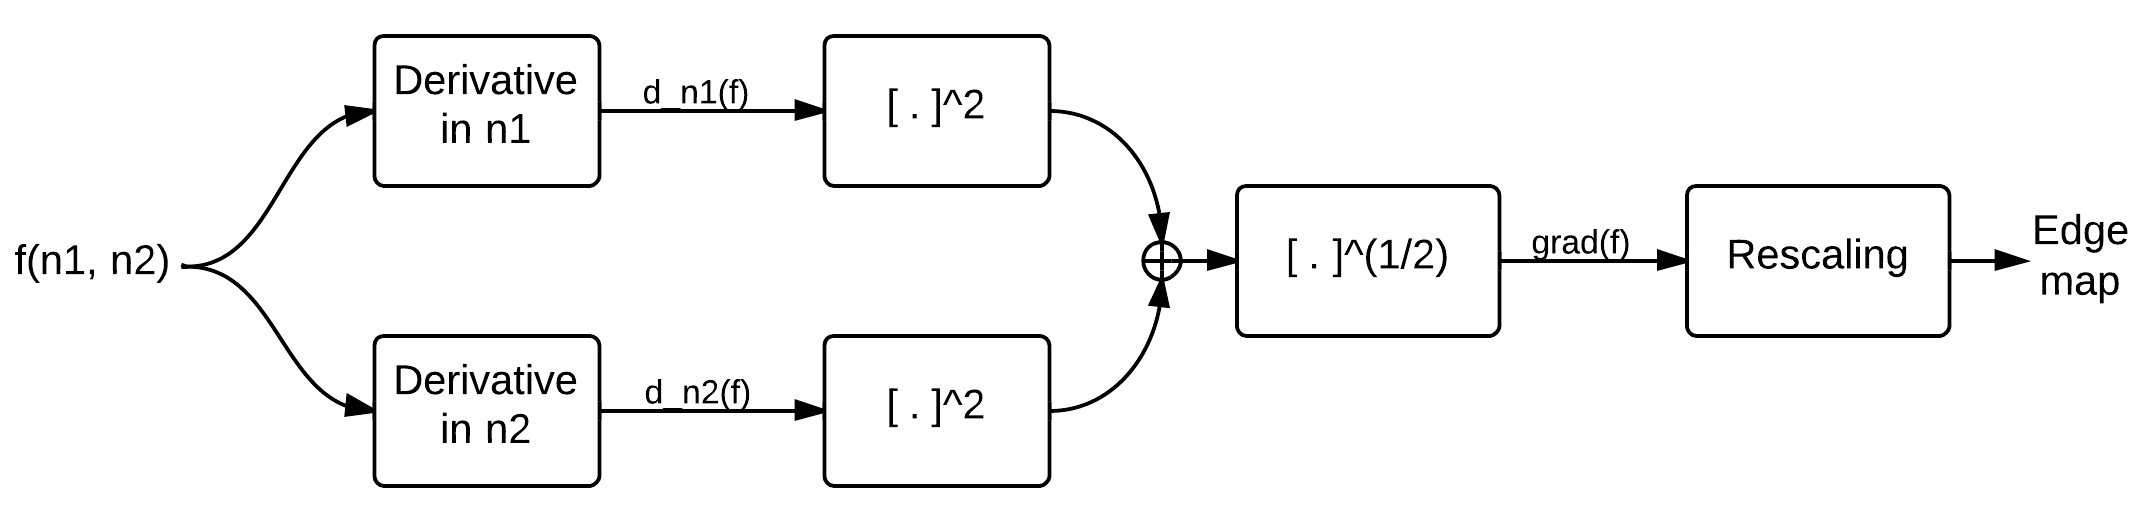
\includegraphics[width=\linewidth]{GradientMethod.png}
\caption{Outline of edge detection using the gradient-based method.}
\label{fig:gradientmethod}
\end{figure}

\section{Laplacian-based method}

The laplacian-based method detects edges in a $2D$ image by finding the analogue of the laplacian for the image and then finding the zero-crossings of the laplacian. Once again, let us think in $1D$ to get an intuition for why this is a sensible thing to do. To find the edges of a $1D$ continuous signal $f(x)$, we would first find the second derivative $\frac{d^2f}{dx^2}$ and then look at its zeros, which correspond to the inflection points of $f(x)$. Here we are defining the edges of $f(x)$ to be its inflection points, which is a reasonable definition. For a 2D continuous signal $f(x,y)$, we can do a very similar thing. We would find the laplacian defined as $\nabla^2f = \frac{\partial^2f}{\partial x^2} +  \frac{\partial^2f}{\partial y^2}$ and search for the zero-crossings. When we are working with a digital image, we are not able to take the laplacian, so we approximate it. Figure \ref{fig:laplacianfilter} presents one filter that can be used to approximate the laplacian.

In Figure  \ref{fig:laplacianmethod}, I present my overall laplacian-based edge detection method. Given an image $f(n_1, n_2)$, we first find the laplacian by using the filter presented in Figure \ref{fig:laplacianfilter}. The standard lapalcian-base method would then proceed to finding the ``zero-crossings." However, I found great difficulty in doing this and defining what a zero-crossing really means for a discrete signal. However I found an alternative approach. After computing the laplacian, I take the absolute value to get the magnitude of the laplacian. I then rescale these values in a completely analogous manner as the way described in the gradient-based method. It is reasonable to consider high values of the laplacian magnitude to indicate edge points because the points around a zero-crossing point (an edge point) tend to have high values. At this point, we do have an edge map, but this edge map looks very noisy. To get rid of most of the false positives, we compute and use an estimate of local variance at each pixel. If the variance is too low at a pixel, then it is not an edge point. Here, we do need a threshold value to determine a variance that is ``too low." I set this threshold to be the $70^{th}$ percentile variance.I reached this value by experimentation.

\begin{figure}
\centering
\begin{tabular}{c || c | c | c }
{\color{light-gray}1} & 1 & 1 & 1 \\
\hline
{\color{light-gray}0} & 1 & -8 & 1 \\
\hline
{\color{light-gray}-1} & 1 & 1 & 1 \\
\hline\hline
& {\color{light-gray}-1} & {\color{light-gray}0} & {\color{light-gray}1} \\
\end{tabular}
\caption{LTI filter to approximate laplacian of a $2D$ discrete signal.}
\label{fig:laplacianfilter}
\end{figure}

\begin{figure}
\centering
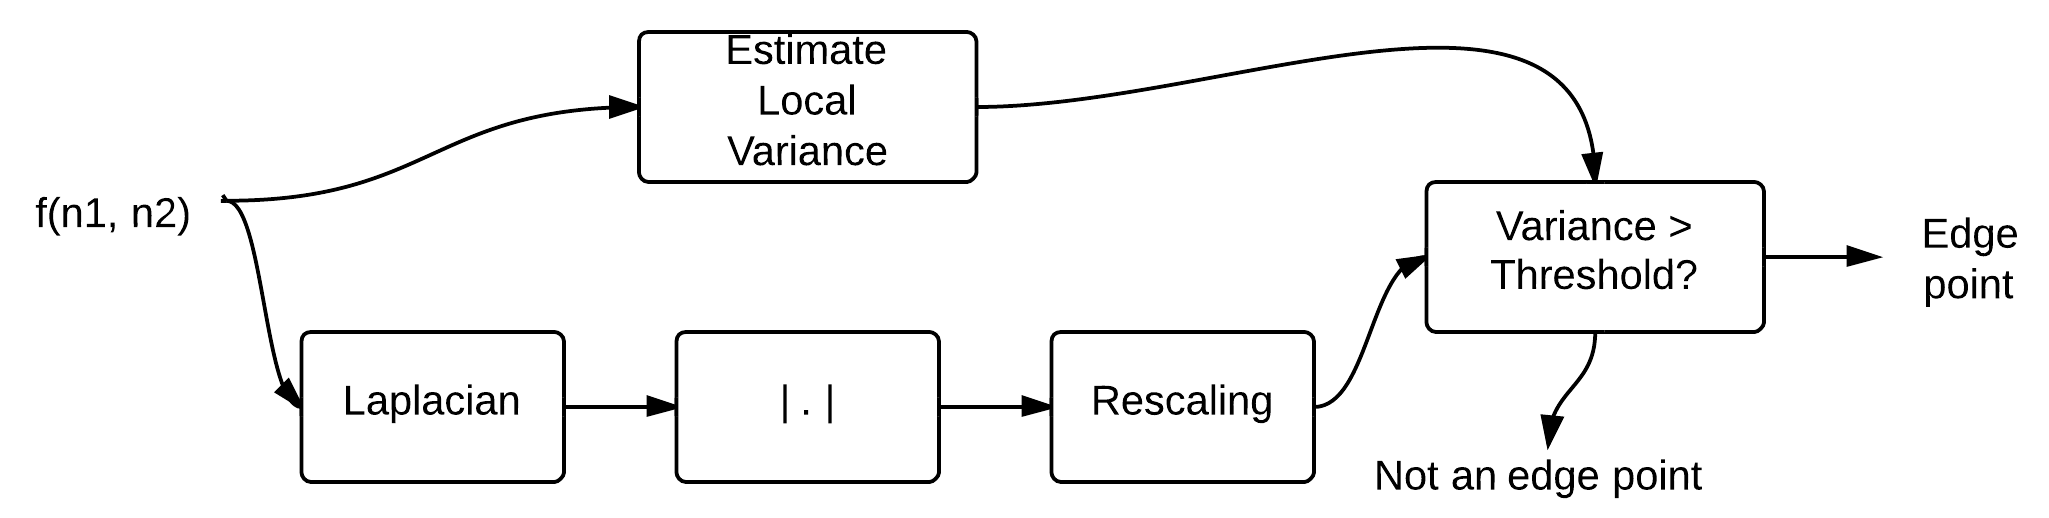
\includegraphics[width=\linewidth]{LaplacianMethod.png}
\caption{Outline of edge detection using the laplacian-based method.}
\label{fig:laplacianmethod}
\end{figure}

\section{Examples}

In Figures \ref{fig:lena} and \ref{fig:stata}, I give two examples of the two methods, first on the famous Lena image, and second on an image of the MIT Stata Building.

\begin{figure}
\setlength{\fboxsep}{0pt}
\minipage{0.32\textwidth}
\fbox{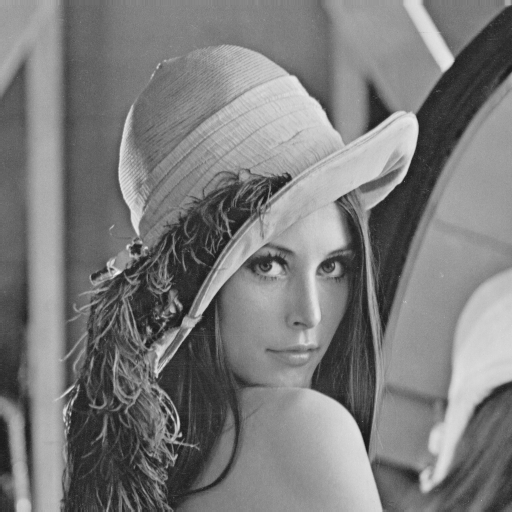
\includegraphics[width=\linewidth]{lena.png}}
\endminipage\hfill
\minipage{0.32\textwidth}
\fbox{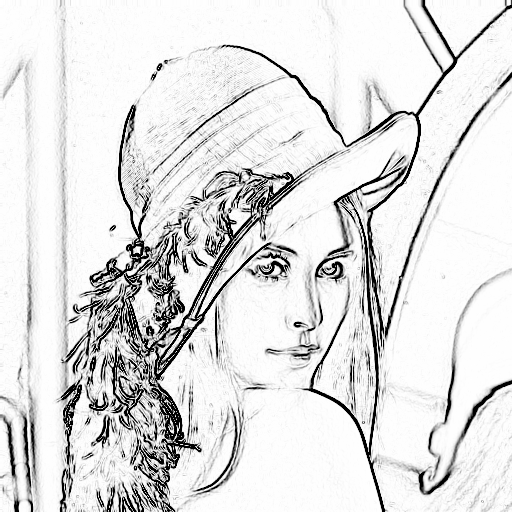
\includegraphics[width=\linewidth]{lena_gradient_edges.png}}
\endminipage\hfill
\minipage{0.32\textwidth}
\fbox{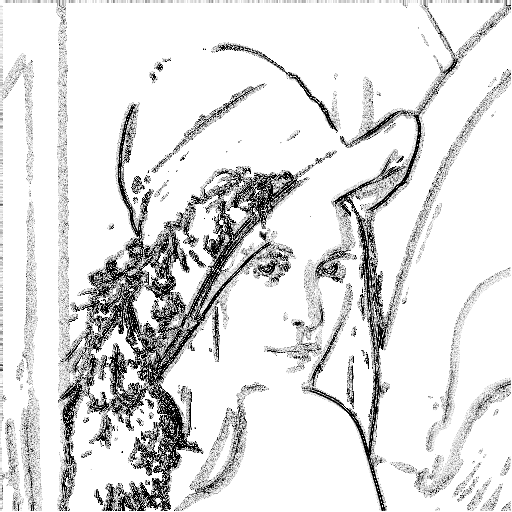
\includegraphics[width=\linewidth]{lena_laplacian_edges.png}}
\endminipage
\caption{Edge detection example: Lena -- original; gradient-based; laplacian-based.}\label{fig:lena}
\end{figure}

\begin{figure}
\setlength{\fboxsep}{0pt}
\minipage{0.32\textwidth}
\fbox{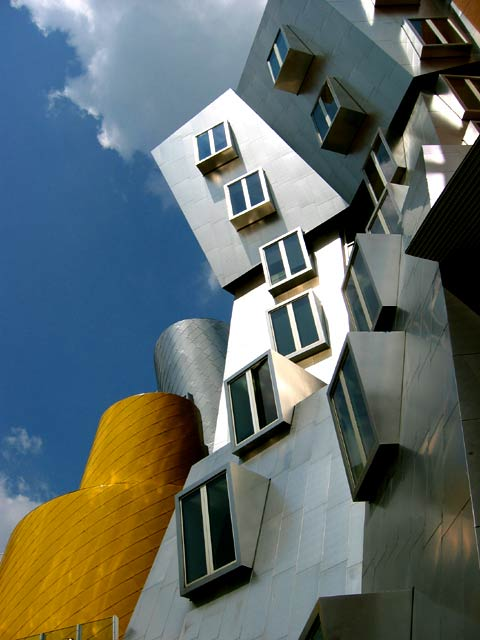
\includegraphics[width=\linewidth]{stata_center.jpg}}
\endminipage\hfill
\minipage{0.32\textwidth}
\fbox{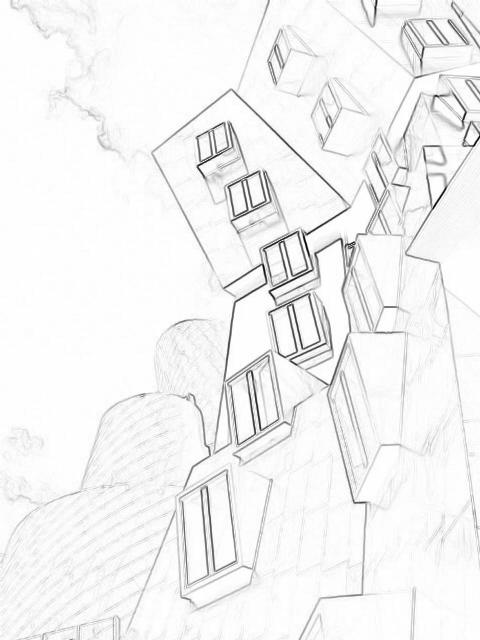
\includegraphics[width=\linewidth]{stata_center_gradient_edges.jpg}}
\endminipage\hfill
\minipage{0.32\textwidth}
\fbox{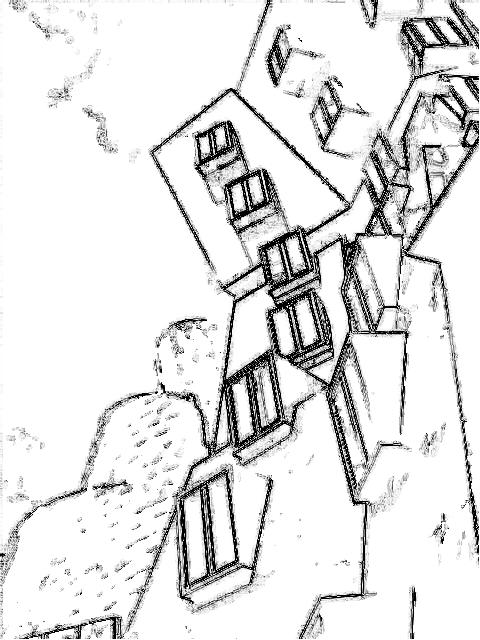
\includegraphics[width=\linewidth]{stata_center_laplacian_edges.jpg}}
\endminipage
\caption{Edge detection example: Stata Center -- original; gradient-based; laplacian-based.}\label{fig:stata}
\end{figure}

\section{Implementation}

I implemented my project completely in the Python programming language. All of my documented code, simple instructions on  how to use it, and additional examples can be found at the project repository: \url{https://github.com/mikemeko/6.344-Project}.

\end{document}
